% !TeX spellcheck = hu_HU
\documentclass[12pt,a4paper]{article}
\usepackage[utf8]{inputenc}
\usepackage{cmap}
\usepackage[T1]{fontenc}
\usepackage[magyar]{babel}
\usepackage{amsmath}
\usepackage{amsfonts}
\usepackage{amssymb}
\usepackage{graphicx}

\usepackage{struktex}
\usepackage{outlines}
\usepackage{hyperref}

\hyphenpenalty=10000

\begin{document}

\begin{center}
	\huge
	Algoritmusok és adatszerkezetek II\\
	\vspace{1mm}
	\LARGE
	Tömörítés témakör jegyzete\\
	\vspace{5mm}
	\large
	Készült Ásványi Tibor előadásai és gyakorlatai alapján\\
	\vspace{5mm}
	Sárközi Gergő, 2021-22-1. félév\\
	Nincsen lektorálva!
\end{center}

\tableofcontents

\pagebreak

\section{Tömörítés}

\begin{outline}
	\1 csak veszteségmentessel foglalkozunk
	\1 kód = kódszavak nemüres halmaza (kódfával ábrázolható)
	\1 betűnkénti kódolás: adatot betűnként
	$ \sum \to \mathbb{C} \subset \mathbb{T}^* $
	bijektív (kölcsönösen egyértelmű) leképezéssel készítjük
		\2 $ \sum $ = ábécé, karakterek halmaza
		\2 $ \mathbb{C} $ = kód
		\2 $ T=\{0,1\} $ általában
		\2 továbbiakban legyen $ r=|\mathbb{T}| $ és $ d=|\sum| $
\end{outline}

\pagebreak

\section{Naiv módszer}

\begin{outline}
	\1 egyenletes kód: kód szavainak hossza egyenlő
	\1 egy karakter (min) $ \lceil log_r d \rceil $ hosszan kódolható
	\1 kódtáblázat: karakter-kód párok
	\1 kódtáblázatot is csatolni kell az adattal
	(és így mérni a tömörítés effektivitását)
\end{outline}

\subsection{Példa}

Bemenet: ERRE\_ARRA\_MERRE\_ARRA \\
$ \sum = \{ E, R, \_, A, M \} \implies d=5 $  \\
$ l=\lceil log_2 5 \rceil=3 $ \\
Kimenet hossza: 20x3=60 + kódtáblázat

\begin{table}[h!]
	\begin{tabular}{|c|c|}
		\hline
		\textbf{Betű} & \textbf{Kód} \\
		\hline
		E & 000 \\
		\hline
		R & 001 \\
		\hline
		\_ & 010 \\
		\hline
		A & 011 \\
		\hline
		M & 100 \\
		\hline
	\end{tabular}
\end{table}

\pagebreak

\section{Huffmann-kód}

\begin{outline}
	\1 betűnkénti optimális kódolás
	\1 2 hiba: 2x kell beolvasni és betűnkénti kódolás (ami pl. képeknél nem nagyon tud tömöríteni)
	\1 nem egyértelmű: azonos gyakoriságú betűk (és 0-1) felcserélhetők
	\1 prefix-kód: kódszavak halmaza prefix mentes
	\1 kódtáblázatot is csatolni kell az adattal
	\1 kódfa: szigorúan bináris fa: 2d-1 csúcs
\end{outline}

\subsection{Példa}

Bemenet: ERRE\_ARRA\_MERRE\_ARRA

\begin{figure}[h]
	\begin{minipage}{.5\textwidth}
		\begin{tabular}{|c|c|}
			\hline
			\textbf{Betű} & \textbf{Gyakoriság} \\
			\hline
			E & 4 \\
			\hline
			R & 8 \\
			\hline
			\_ & 3 \\
			\hline
			A & 4 \\
			\hline
			M & 1 \\
			\hline
		\end{tabular}
	\end{minipage}
	\begin{minipage}{.5\textwidth}
		\begin{tabular}{|c|}
			\hline
			\textbf{minPrQueue} \\
			\hline
			<(1,M),(3,\_),(4,A),(4,E),(8,R)> \\
			\hline
			<(4,M\_),(4,A),(4,E),(8,R)> \\
			\hline
			<(4,E),(8,R),(8,M\_A)> \\
			\hline
			<(8,M\_A),(12,ER)> \\
			\hline
			<(20,M\_AER)> \\
			\hline
		\end{tabular}
	\end{minipage}
\end{figure}

\begin{outline}
	\1 amíg a sorban van $\ge2$ elem
	\2 szedjük ki őket, készítsünk egy szülő node-ot nekik (bal/jobb oldalt kapja egy gyerek a gyakorisága alapján)
	\2 rakjuk be a szülő node-ot a gyerekek értékének összértékével
	\1 kész a fa
\end{outline}

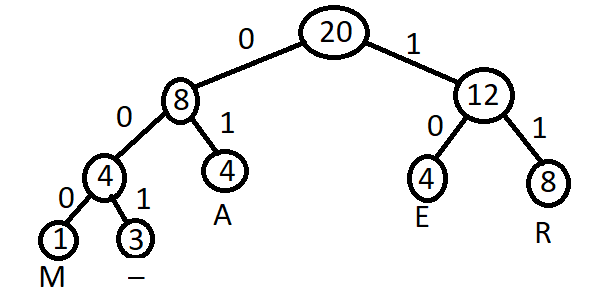
\includegraphics[width=0.7\linewidth]{huffman-code-tree}

TODO stuki (kóddal együtt - kóddal tesztelve)

\pagebreak

\section{Lempel-Ziv-Welch (LZW) módszer}

\begin{outline}
	\1 nem betűnkénti kódolás: szótárkód
		\2 nincs meg az a hatékonysági határ, mint Huffmann kódnál
	\1 lépésről lépésre egy $S$ kódtáblát (szótárat) bővít
	\1 szótár tulajdonságai:
		\2 egybetűs szavak alapból szerepelnek benne
		\2 ha egy szó benne van a szótárban, akkor minden kezdődarabja is benne van
		\2 minden tárolt szónak ($x \in S$) fix hosszúságú kódja van ($c(x)$)
	\1 csak egyszer olvassuk be az adatot: egy időben kódolunk és építünk szótárat
	\1 kódtáblát nem kell csatolni a kódolt adathoz
	\1 kódolás: ha $x \in S$ szót találunk és a következő betű, $Y$, már $\notin S$,
	akkor $c(x)$-et kiírjuk, $xY$ szót felvesszük a $S$ szótárba. $c(xY)$ a legkisebb szabad kód.
	A beolvasást az $Y$ betűvel folytatjuk.
	\1 $c(x)$ fix hosszú, méghozzá ez a hossz egy előre ismert konstans (általában 12 bit)
	\1 a kódolt adat mellé nem szükséges a szótár csatolása
	\1 hibák:
		\2 hosszú szöveg esetén túl sok új kód van bevezetve, ami lassít
		\2 ezért korlátozhatjuk a kódszavak számát, hosszát
		\2 vagy csak a bemenet egy kezdőszeletén építjük a szótárat, utána már csak használjuk
	\1 Kódot egyből felhasználjuk miután berakjuk szótárba:
	nem probléma, így is ki tudjuk találni a kód utolsó karakterét: azonos az elsővel
\end{outline}

\pagebreak

\subsection{Példa}

\begin{figure}[h]
	\begin{minipage}{.5\textwidth}
		\begin{tabular}{|c|c|c|c|}
			\hline
			\multicolumn{4}{|c|}{Bemenet: BBCABCABABAAC} \\
			\hline
			Ki  & Akt. & Köv. & Új \\
			kód & szó & szó & kód \\
			\hline
			2 & B & B & 4 \\
			\hline
			2 & B & C & 5 \\
			\hline
			3 & C & A & 6 \\
			\hline
			1 & A & B & 7 \\
			\hline
			5 & BC & A & 8 \\
			\hline
			7 & AB & A & 9 \\
			\hline
			9 & ABA & A & 10 \\
			\hline
			1 & A & C & 11 \\
			\hline
			3 & C & - & - \\
			\hline
		\end{tabular}
		\caption{Kódolás példa}
	\end{minipage}
	\begin{minipage}{.5\textwidth}
		\begin{tabular}{|c|c|c|c|}
			\hline
			\multicolumn{4}{|c|}{Bemenet: 2 2 3 1 5 7 9 1 3} \\
			\hline
			Be  & Akt. & Köv. & Új \\
			kód & szó & szó & kód \\
			\hline
			2 & B & B & 4 \\
			\hline
			2 & B & C & 5 \\
			\hline
			3 & C & A & 6 \\
			\hline
			1 & A & B & 7 \\
			\hline
			5 & BC & A & 8 \\
			\hline
			7 & AB & A & 9 \\
			\hline
			9 & ABA & ... & 10 \\
			\hline
			... & ... & ... & ... \\
			\hline
			... & ... & ... & ... \\
			\hline
		\end{tabular}
		\caption{Dekódolás példa}
	\end{minipage}
\end{figure}

\pagebreak

\subsection{Stuki}

\begin{outline}
	\1 Ha a kódok $b$ bitesek, akkor $MAXCODE = 2^b-1$
	\1 Item: szó-kód pár ($string:\sum <>$ és $code:\mathbb{N}$ pár)
\end{outline}

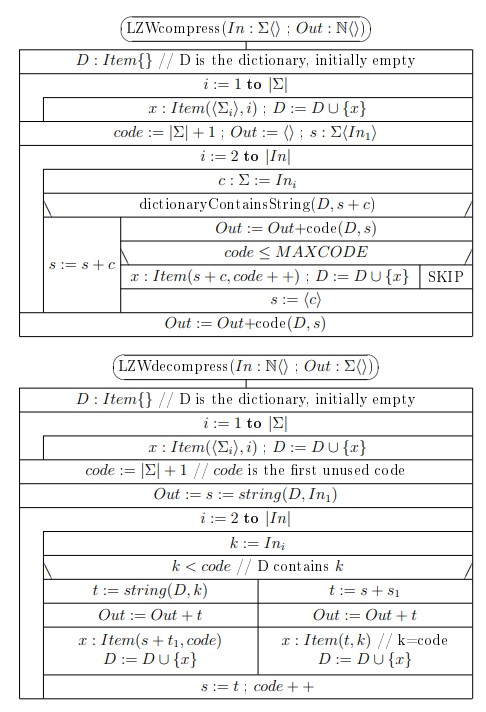
\includegraphics[width=0.8\linewidth]{lzw}

\end{document}
